\documentclass[a4paper,12pt]{scrbook}

\usepackage[utf8]{inputenc}
\usepackage[ngerman]{babel}
\usepackage[T1]{fontenc}
\usepackage{amsmath}
\usepackage{graphicx}


\title{Diplomarbeit}
\author{Dominik Pichler}
\date{21. Jänner 2018}

\begin{document}

\maketitle
\tableofcontents

\section{Teil 1 Mechanik}
\subsection{Einleitung}
\subsubsection{Aufgabenstellung}
\subsubsection{Zielsetzung}
\subsubsection{Problematik}
\subsection{Konzepte}
\subsubsection{Variante 1}

\begin{figure}
\begin{center}
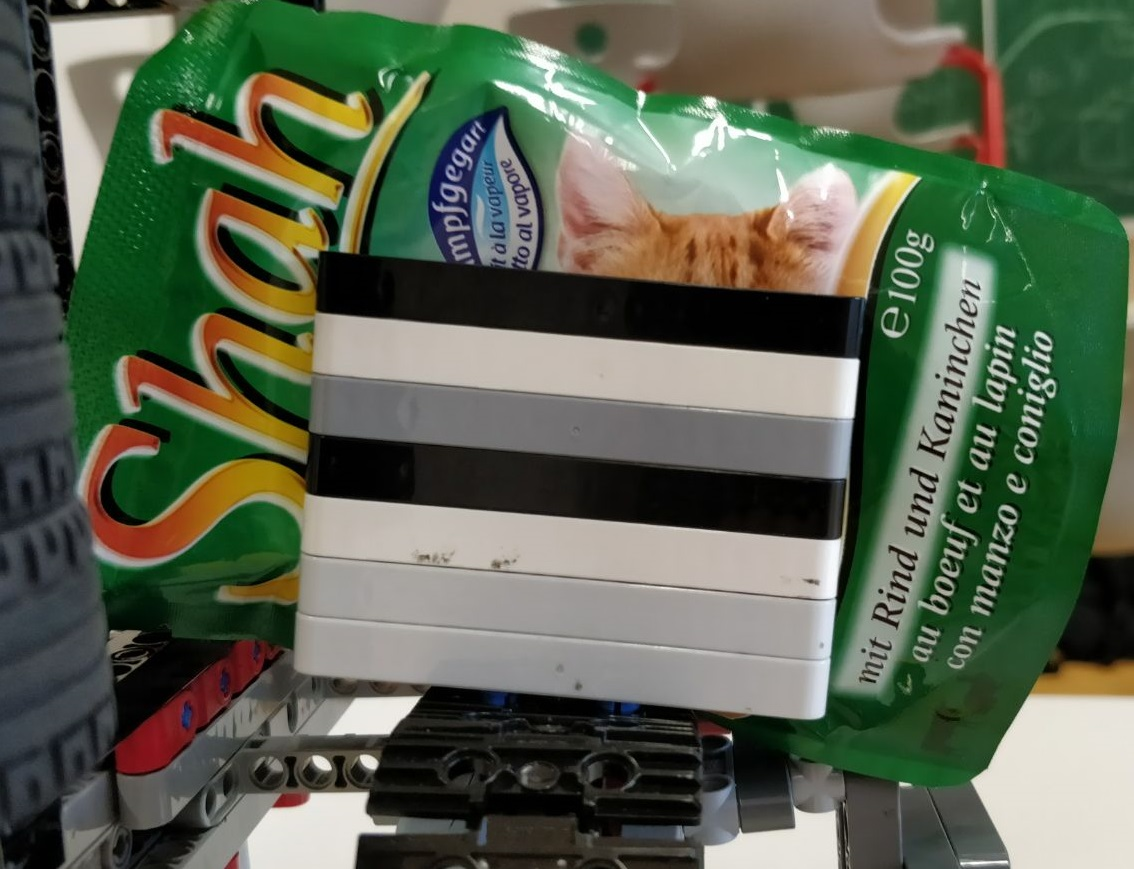
\includegraphics[width=4]{Magazin_Vorne.jpeg}
\caption{Magazin_Vorne}
\end{center}
\end{figure}

\subsection{Aufbauten und Tests}
\subsection{Vergleich der Varianten}
\subsection{Konstruktion der Wahlvariante und Details}
\subsection{Berechnung und Dimensionierung}
\subsection{Simulation}
\subsection{Bedienung und Wartung}
\subsection{Selbstkritische Analyse und Ausblick}


\end{document}
